% INF-TEST-MS-01: evidencia integral multifuente para la tesis.
\documentclass[11pt,letterpaper]{article}
\usepackage[utf8]{inputenc}
\usepackage[T1]{fontenc}
\usepackage[spanish,es-nodecimaldot]{babel}
\usepackage[letterpaper,margin=2.1cm,headheight=15pt]{geometry}
\usepackage[protrusion=true,expansion=false]{microtype}
\usepackage{xcolor}
\usepackage{booktabs}
\usepackage{tabularx}
\usepackage{longtable}
\usepackage{array}
\usepackage{enumitem}
\usepackage{graphicx}
\usepackage{adjustbox}
\usepackage{fancyhdr}
\usepackage{hyperref}
\usepackage{xurl}
\usepackage{caption}
\usepackage{float}

\ifdefined\pdfinfoomitdate\pdfinfoomitdate=1\fi
\ifdefined\pdftrailerid\pdftrailerid{}\fi
\ifdefined\pdfsuppressptexinfo\pdfsuppressptexinfo=15\fi

\definecolor{ugblue}{HTML}{006A8D}
\definecolor{deepgreen}{HTML}{123D3A}
\definecolor{softgray}{HTML}{F1F5F4}
\definecolor{success}{HTML}{157A57}
\definecolor{warning}{HTML}{A45A00}
\definecolor{danger}{HTML}{A83224}
\hypersetup{
  colorlinks=true,
  linkcolor=ugblue,
  urlcolor=ugblue,
  hypertexnames=false,
  pdftitle={Informe de pruebas integrales multifuente BI mas IA},
  pdfauthor={Emily Dayan Robles Alvarado y Lesly Samay Velasquez Anchundia}
}

\pagestyle{fancy}
\fancyhf{}
\lhead{Pruebas integrales multifuente}
\rhead{Prototipo BI asistido por IA}
\cfoot{\thepage}
\setlength{\parindent}{0pt}
\setlength{\parskip}{0.48em}
\setlength{\emergencystretch}{2em}
\setlist[itemize]{leftmargin=1.5em,itemsep=0.18em}
\setlist[enumerate]{leftmargin=1.7em,itemsep=0.22em}
\renewcommand{\arraystretch}{1.18}
\newcommand{\file}[1]{\texttt{#1}}
\newcommand{\ok}{\textcolor{success}{\textbf{Aprobado}}}
\newcommand{\fixed}{\textcolor{ugblue}{\textbf{Verificado}}}
\newcommand{\notebox}[1]{\begin{center}\fcolorbox{ugblue}{softgray}{\begin{minipage}{0.91\textwidth}\textcolor{ugblue}{\textbf{Criterio de interpretación.}} #1\end{minipage}}\end{center}}

\begin{document}
\hypersetup{pageanchor=false}
\begin{titlepage}
  \thispagestyle{empty}
  \vspace*{0.7cm}
  {\color{ugblue}\rule{\textwidth}{2.8pt}}
  \vspace{1.1cm}
  {\Large Universidad de Guayaquil\\[0.2em]
  Facultad de Ciencias Matemáticas y Físicas\\
  Carrera de Software}
  \vfill
  {\color{deepgreen}\fontsize{24}{30}\selectfont\textbf{Informe de pruebas integrales}}\\[0.6em]
  {\LARGE Validación multifuente del flujo BI asistido por IA}\\[0.65em]
  {\large AdventureWorks 2022 y WideWorldImporters\\
  desde metadatos hasta analítica y reportería\par}
  \vspace{1.3cm}
  \begin{tabularx}{\textwidth}{@{}>{\bfseries}l X@{}}
    Autoras & Emily Dayan Robles Alvarado y Lesly Samay Velásquez Anchundia \\
    Código documental & INF-TEST-MS-01 \\
    Versión & 1.0.0 \\
    Fecha de ejecución & 1 de octubre de 2026 \\
    Incremento evaluado & Sprint 6 -- contexto multifuente universal para SQL Server \\
    Rama evaluada & \file{feature/multi-source-sqlserver} \\
    Estado & Pruebas funcionales, automatizadas y documentales aprobadas \\
  \end{tabularx}
  \vfill
  {\color{ugblue}\rule{\textwidth}{2.8pt}}
\end{titlepage}

\hypersetup{pageanchor=true}
\pagenumbering{roman}
\tableofcontents
\newpage
\listoftables
\listoffigures
\newpage
\pagenumbering{arabic}

\section{Propósito académico y alcance}

Este informe reúne evidencia reproducible para sustentar que el prototipo puede operar dos
fuentes SQL Server con estructuras distintas sin mezclar sus metadatos, catálogos,
propuestas, ejecuciones ni resultados analíticos. La evaluación cubre el recorrido visible
al analista: selección de fuente, exploración de esquema, catálogo, expedientes de
datamart, ejecución ETL ya conciliada, tablero, copiloto contextual y exportaciones PDF y
Excel.

El estudio usa AdventureWorks 2022 y WideWorldImporters como casos de contraste. No son
dos implementaciones específicas: ambas atraviesan los mismos servicios de introspección,
resolución semántica, validación, materialización y analítica. Las diferencias observadas
---por ejemplo, territorios comerciales en AdventureWorks y estados en
WideWorldImporters--- proceden de la evidencia de cada esquema.

\notebox{La conclusión se limita al alcance probado: múltiples fuentes SQL Server y el
dominio ventas. No demuestra todavía portabilidad a MySQL, combinación de hechos entre
bases ni validez estadística para todo esquema empresarial posible.}

\section{Método de prueba}

Se aplicó una estrategia de triangulación con cuatro capas:

\begin{enumerate}
  \item \textbf{Prueba automatizada:} contratos de backend, interfaz, aislamiento,
  recuperación, exportación y compilación estricta.
  \item \textbf{Prueba funcional de caja negra:} recorrido del sistema desde la interfaz,
  alternando la fuente sin cerrar sesión.
  \item \textbf{Conciliación:} comparación de filas y medidas de origen frente al datamart
  materializado.
  \item \textbf{Inspección de artefactos:} renderizado página por página de PDF y lectura
  estructural y visual de Excel.
\end{enumerate}

Las incidencias encontradas se trataron como resultados de prueba: se documentó el síntoma,
se identificó la causa, se añadió una corrección común y se repitió el escenario. No se
alteraron los resultados para ocultar fallos.

\subsection{Entorno evaluado}

\begin{table}[H]
\centering
\caption{Entorno técnico de ejecución}
\begin{tabularx}{\textwidth}{@{}p{0.27\textwidth}X@{}}
\toprule
Componente & Configuración observada \\
\midrule
Aplicación & React/Vite y FastAPI ejecutados mediante Docker Compose \\
Persistencia de control & PostgreSQL con migraciones Alembic hasta \file{20261001\_18} \\
Fuentes & SQL Server: AdventureWorks2022 y WideWorldImporters \\
Proveedor visible & Anthropic Claude Haiku 4.5 en las consultas contextuales repetidas \\
Navegador & Navegador integrado, sesión de Administrador inicial \\
Fecha & 1 de octubre de 2026, zona America/Guayaquil \\
\bottomrule
\end{tabularx}
\end{table}

\section{Matriz de escenarios y criterios}

\begin{longtable}{@{}p{0.09\textwidth}p{0.25\textwidth}p{0.39\textwidth}p{0.13\textwidth}@{}}
\caption{Escenarios integrales ejecutados}\label{tab:escenarios}\\
\toprule
ID & Escenario & Evidencia esperada & Resultado \\
\midrule
\endfirsthead
\toprule
ID & Escenario & Evidencia esperada & Resultado \\
\midrule
\endhead
MS-E2E-01 & Cambiar de fuente en Inicio & Nombre, base e instantánea corresponden a la fuente elegida. & \ok \\
MS-E2E-02 & Explorar metadatos & Las cifras, tablas y versión se reinician; no queda detalle de la fuente previa. & \ok \\
MS-E2E-03 & Revisar catálogo & Cada fuente conserva orientación propia y sólo usa evidencia de su instantánea. & \ok \\
MS-E2E-04 & Consultar expedientes & Propuestas y ejecuciones visibles pertenecen a la conexión seleccionada. & \ok \\
MS-E2E-05 & Abrir analítica & KPI, filtros, productos y territorios proceden del datamart correcto. & \ok \\
MS-E2E-06 & Interactuar y alternar & Un punto seleccionado en una fuente no persiste al cambiar a la otra. & \ok \\
MS-E2E-07 & Consultar al copiloto & ``Territorio líder'' se resuelve contra el ranking verificado de la fuente activa. & \ok \\
MS-E2E-08 & Exportar PDF y Excel & El contenido conserva fuente, ejecución, filtros y maquetación legible. & \ok \\
MS-E2E-09 & Verificar propuestas históricas & Consultar o reconstruir evidencia no cambia el estado; Datamart y Analítica muestran la misma ejecución y propuesta publicadas. & \ok \\
\bottomrule
\end{longtable}

\section{Resultados por fuente}

\subsection{Metadatos y catálogo}

\begin{table}[H]
\centering
\caption{Evidencia estructural independiente por conexión}
\begin{tabularx}{\textwidth}{@{}Xrrrrr@{}}
\toprule
Fuente & Instantánea & Esquemas & Tablas & Columnas & Relaciones \\
\midrule
AdventureWorks2022 & 2 (\file{bf2842f08c8f}) & 6 & 71 & 482 & 90 \\
WideWorldImporters & 3 (\file{008c4832c216}) & 4 & 48 & 546 & 98 \\
\bottomrule
\end{tabularx}
\end{table}

AdventureWorks conservó seis preguntas: las cuatro preguntas estándar y las dos agregadas
por el analista sobre costos/rentabilidad y ventas/costos por unidad. WideWorldImporters
mostró sus cuatro preguntas estándar sin heredar la personalización de AdventureWorks.
La IA interpreta la necesidad y propone; el catálogo funcional y la aceptación técnica
siguen bajo control de la plataforma y del analista.

\begin{figure}[H]
\centering
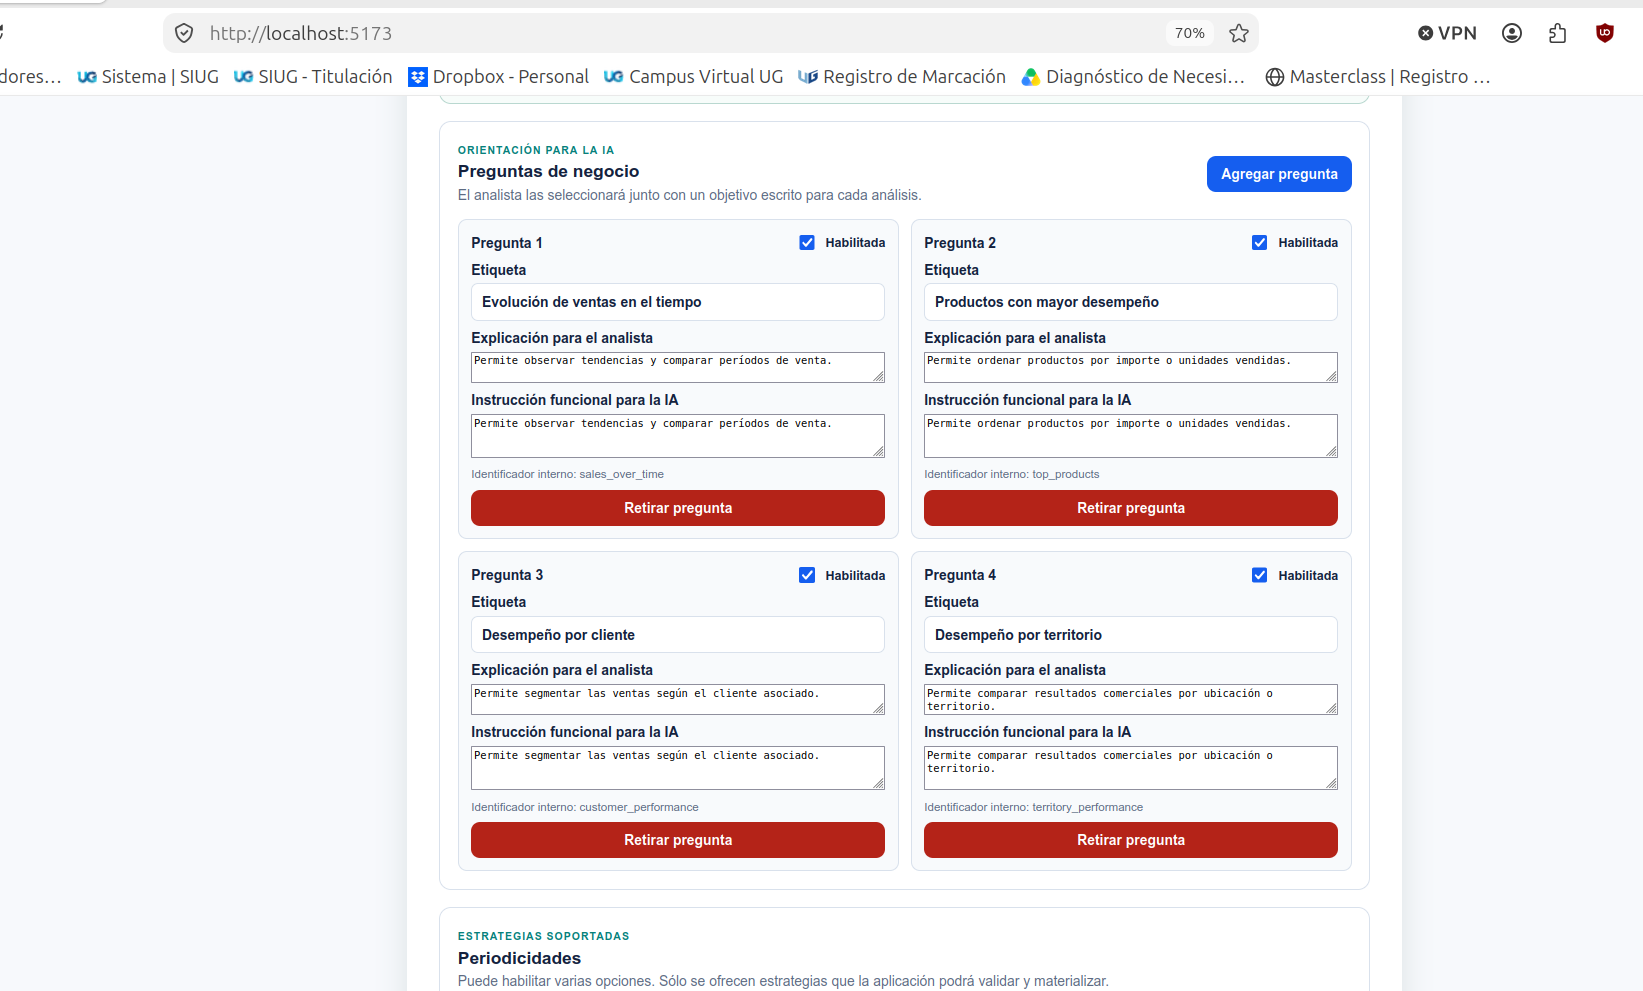
\includegraphics[width=0.94\textwidth]{evidencias/incidencia-catalogo-adventureworks.png}
\caption{Evidencia inicial usada para detectar la pérdida de preguntas personalizadas.}
\end{figure}

\subsection{ETL y conciliación}

\begin{table}[H]
\centering
\caption{Conciliación de las ejecuciones publicadas}
\begin{tabularx}{\textwidth}{@{}Xrrrrl@{}}
\toprule
Fuente & Propuesta & Ejecución & Origen & Datamart & Estado \\
\midrule
AdventureWorks2022 & 91 & 12 & 121.317 & 121.317 & diferencia 0 \\
WideWorldImporters & 96 & 13 & 231.412 & 231.412 & diferencia 0 \\
\bottomrule
\end{tabularx}
\end{table}

Los esquemas físicos son distintos (\file{mart\_ventas\_e12} y
\file{mart\_ventas\_e13}). La ejecución 12 conserva 31.465 pedidos y la ejecución 13
73.595. En ambos casos el registro de reconciliación declara \file{passed=true}; no se
detectaron filas rechazadas ni diferencia de conteo.

\subsection{Analítica y semántica territorial}

AdventureWorks presentó Southwest como territorio líder y productos de bicicletas, con
venta total de 109.846.381,40 USD. WideWorldImporters presentó Texas como territorio líder
y productos de embalaje, con ventas de 177.634.276,40 en moneda de origen. La etiqueta
genérica evita asignar una divisa ISO que la fuente no demuestra de forma inequívoca.

La diferencia Southwest--Texas no constituye una inconsistencia. Es la consecuencia
correcta de dos modelos operacionales diferentes: AdventureWorks expone territorios
comerciales y WideWorldImporters permite derivar estados mediante relaciones verificadas.

\subsection{Inmutabilidad de la verificación histórica}

La repetición del escenario MS-E2E-09 reprodujo un defecto de trazabilidad: la acción de
consulta comparaba la huella de una propuesta histórica con la reconstrucción del motor
vigente y retiraba automáticamente la aprobación cuando ambas diferían. Las propuestas 91
y 86 cambiaron de estado aunque sus ejecuciones 12 y 11 ya estaban conciliadas. La causa
no estaba en los datos ni en el ETL, sino en un efecto lateral indebido de la verificación.

\begin{figure}[H]
\centering
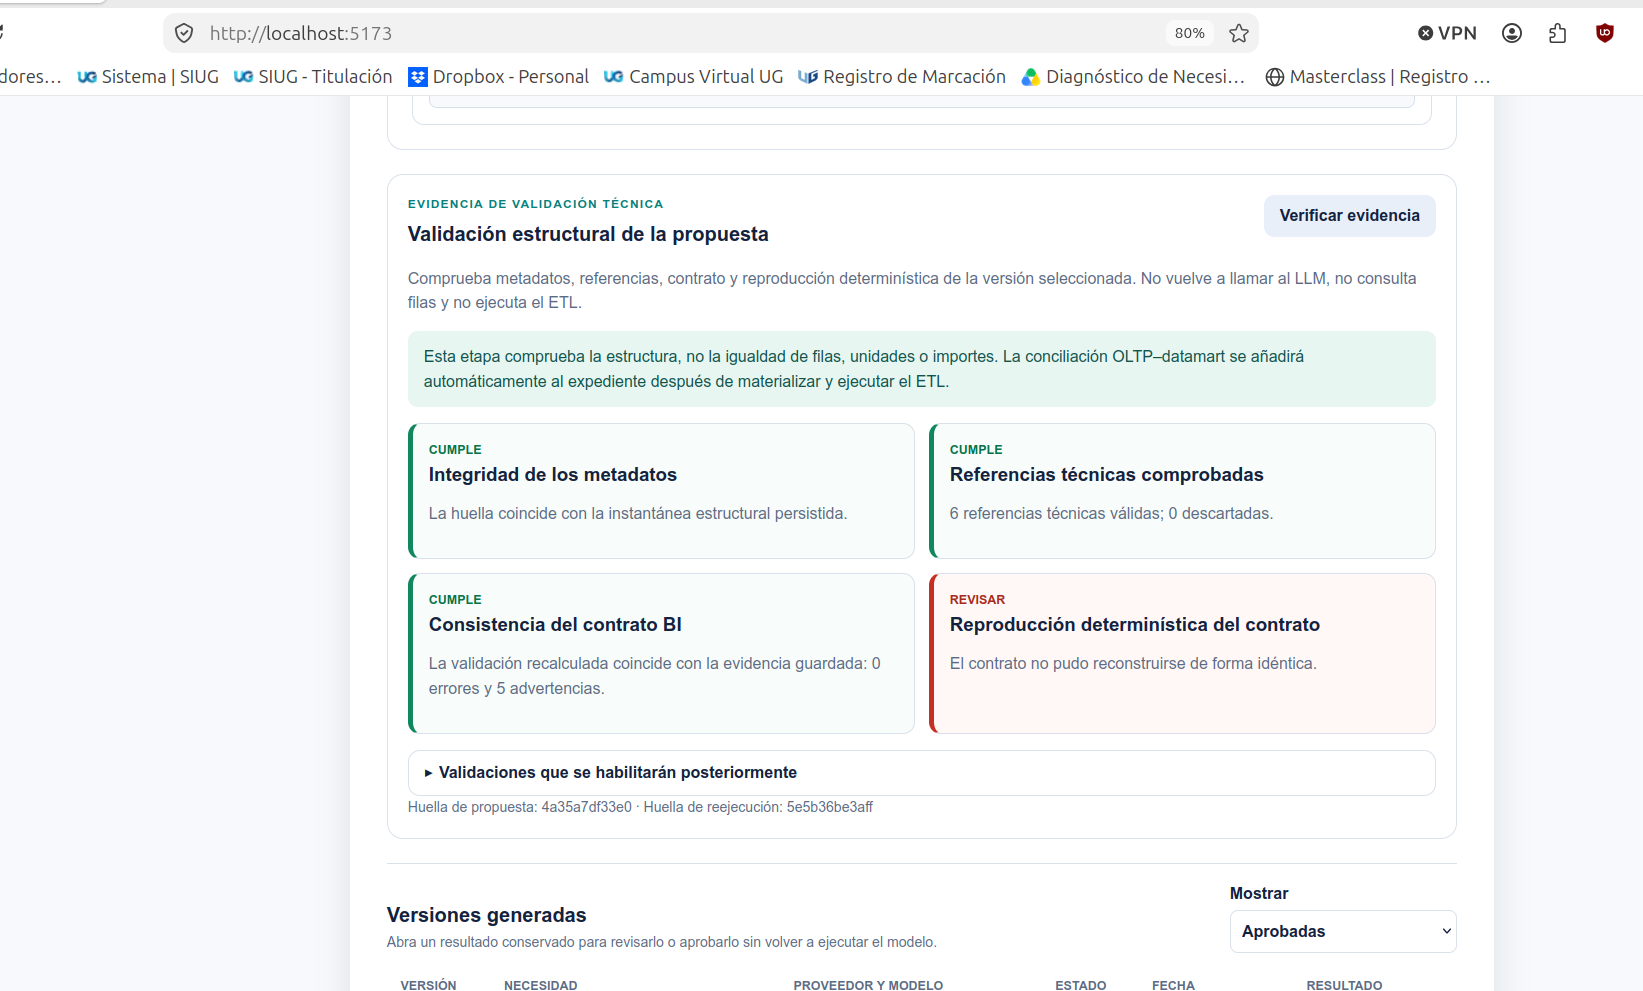
\includegraphics[width=0.94\textwidth]{evidencias/incidencia-verificacion-historica.png}
\caption{Incidencia: una diferencia de reconstrucción histórica aparecía como revisión bloqueante.}
\end{figure}

La corrección separó tres conceptos: validez estructural vigente, reproducción histórica y
estado aprobado. \textbf{Verificar evidencia} es ahora una operación de sólo lectura; una
diferencia de huella se conserva como advertencia de compatibilidad y sólo los errores
actuales de instantánea, referencia o contrato impiden una ejecución nueva. La migración
\file{20261001\_18} restauró exclusivamente las aprobaciones retiradas por el mensaje
automático anterior que además tenían una ejecución conciliada, y registró un evento de
auditoría por propuesta. Después de volver a verificar la versión 91, PostgreSQL conservó
\file{status=approved} y el evento registró \file{status\_unchanged=true}.

La segunda inconsistencia era visual: la pantalla de materialización elegía una propuesta
aprobada no ejecutada como contexto inicial, mientras Analítica leía la ejecución publicada
más reciente. Ahora Datamart abre primero el último expediente conciliado. Para
AdventureWorks ambas vistas identificaron ejecución 12 y propuesta 91; la propuesta 72
permanece disponible sólo como alternativa para una materialización nueva.

\begin{figure}[H]
\centering
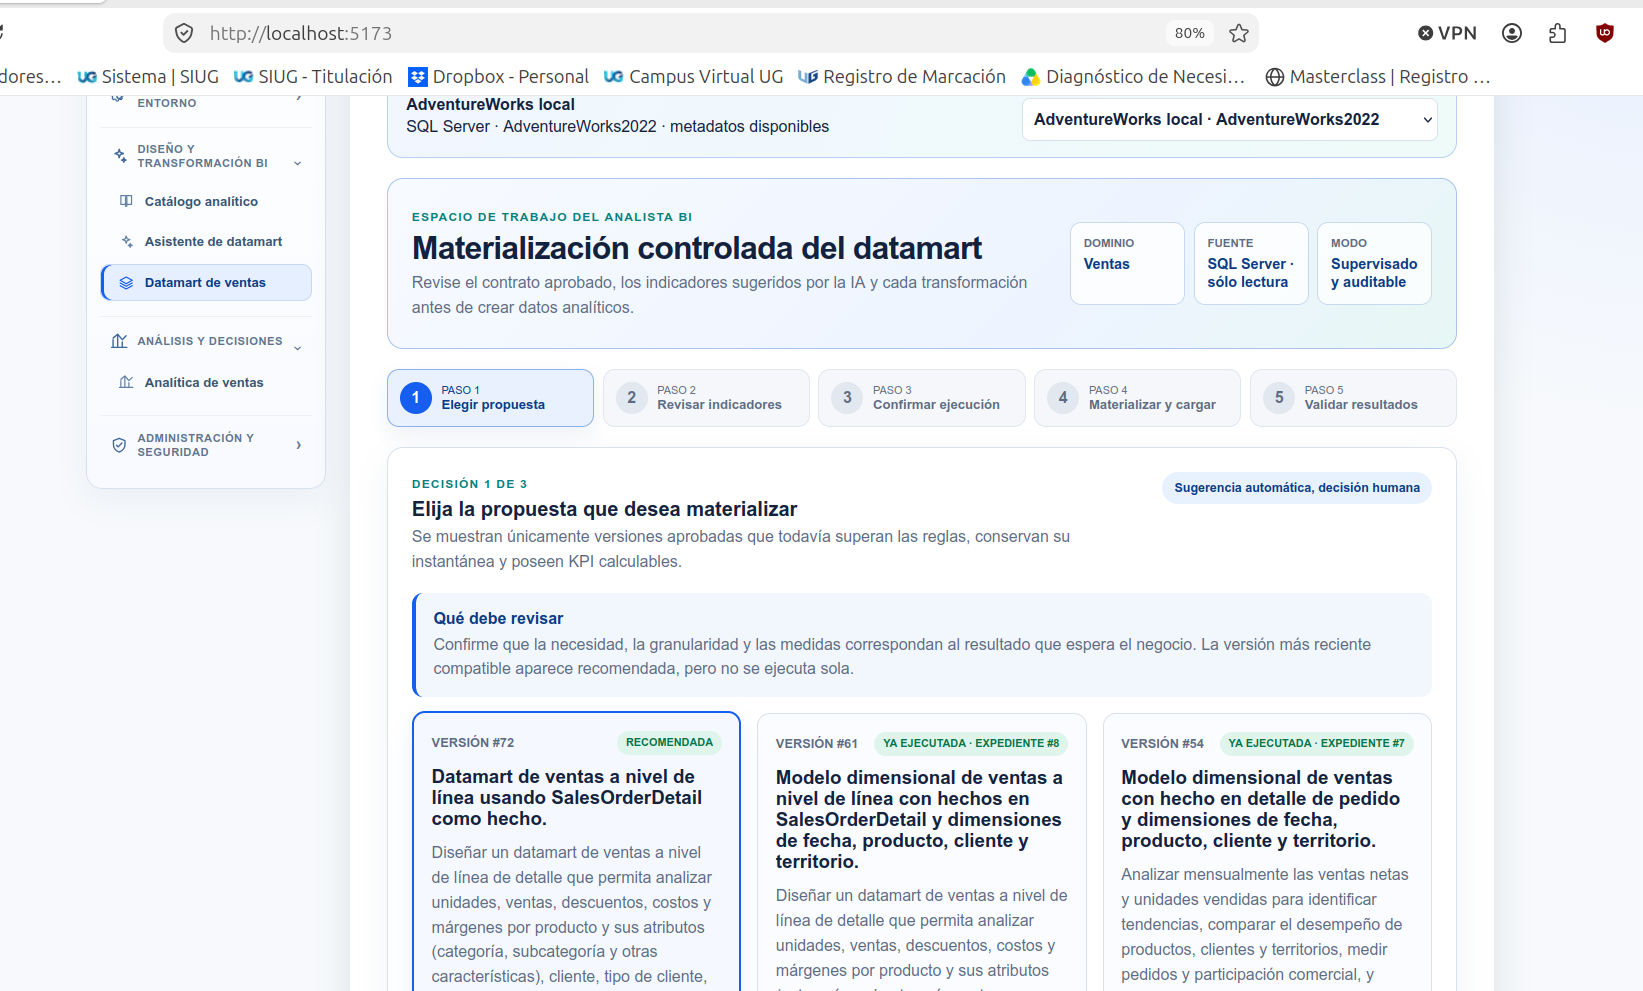
\includegraphics[width=0.94\textwidth]{evidencias/incidencia-contexto-datamart.png}
\caption{Incidencia previa: una propuesta no ejecutada aparecía como recomendada aunque el tablero procedía de la propuesta 91.}
\end{figure}

\section{Aislamiento al alternar fuentes}

La prueba alternó AdventureWorks, WideWorldImporters y nuevamente AdventureWorks sin
cerrar sesión. Se comprobaron los siguientes invariantes:

\begin{itemize}
  \item Inicio cambió nombre, base e instantánea de disponibilidad;
  \item el Explorador reconstruyó su estado y mantuvo visible el selector de versión,
  incluso cuando sólo existía una instantánea;
  \item una respuesta tardía de la fuente anterior no pudo sobrescribir la vista nueva;
  \item la lista analítica mostró únicamente ejecuciones de la conexión activa;
  \item filtros y selección interactiva se limpiaron durante la transición;
  \item productos, territorios y KPI nunca coexistieron con etiquetas de la otra fuente.
\end{itemize}

\begin{figure}[H]
\centering
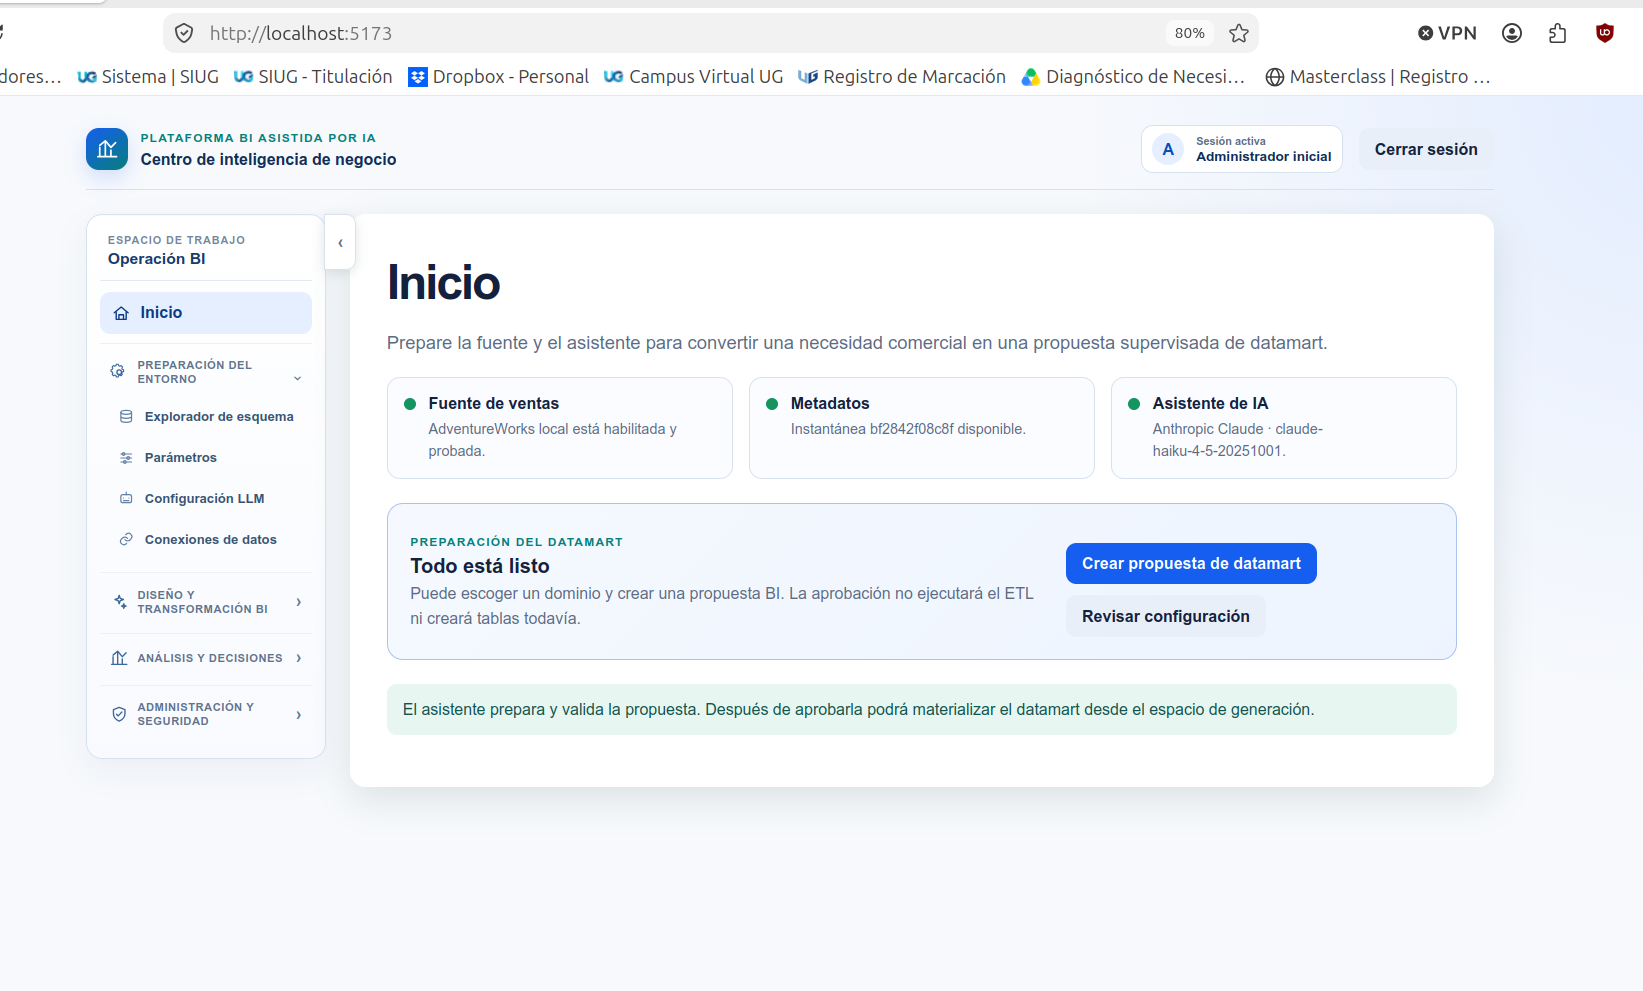
\includegraphics[width=0.92\textwidth]{evidencias/incidencia-inicio-contexto.png}
\caption{Incidencia de contexto inicial que motivó la prueba de aislamiento en Inicio.}
\end{figure}

\begin{figure}[H]
\centering
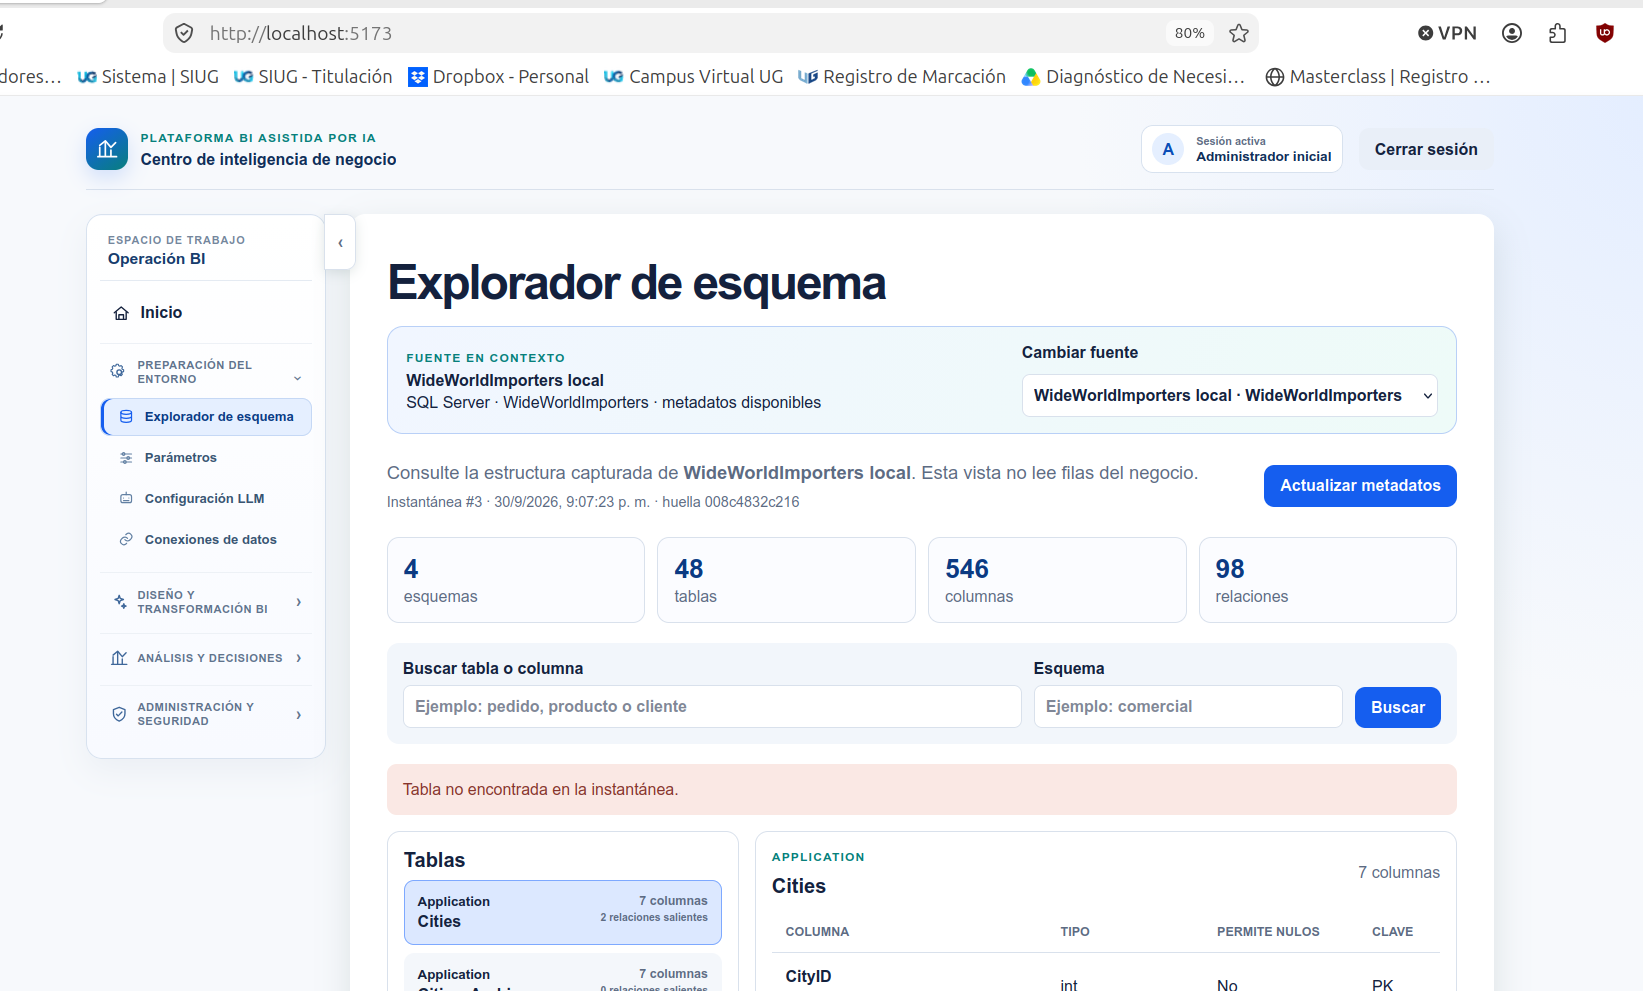
\includegraphics[width=0.92\textwidth]{evidencias/incidencia-explorador-version.png}
\caption{Incidencia de UX del selector de versión en WideWorldImporters.}
\end{figure}

\section{Copiloto contextual y neutralidad del modelo}

La pregunta ``¿Cuáles son los 5 productos con mayor resultado en el territorio líder?''
reveló una ambigüedad: un LLM podía reconocer la intención general pero omitir el filtro
territorial en el objeto estructurado. La corrección no se incorporó al prompt de un modelo
específico. La plataforma ahora detecta el concepto ``territorio líder'', obtiene ese valor
del ranking conciliado vigente y completa el filtro antes de ejecutar la agregación segura.

La repetición produjo:

\begin{itemize}
  \item En la primera fuente: alcance Southwest, cinco productos de AdventureWorks y
  denominador de 24.184.609,60 USD.
  \item En la segunda fuente: alcance Texas, cinco productos de WideWorld Importers y
  denominador de 12.328.671,15 en moneda de origen.
\end{itemize}

Este control es independiente de Groq o Claude: el LLM interpreta, pero no decide qué valor
es líder ni ejecuta SQL libre. La aplicación resuelve el filtro con datos de la ejecución
activa y consulta únicamente agregaciones permitidas.

\notebox{En esta ronda se repitió el copiloto con Claude Haiku 4.5. La comparativa de Groq y
Claude, incluidos rechazos de contrato, límites y niveles de razonamiento, permanece en el
experimento documental del 27 de septiembre. No se presenta esta ronda como una nueva
comparación estadística de proveedores.}

\section{Reportería PDF y Excel}

Se descargaron reportes ejecutivos para las ejecuciones 12 y 13. Cada PDF contiene cinco
páginas: portada/KPI, tendencia, productos, territorios y hallazgos. Se renderizaron todas
las páginas con Poppler. Los valores extensos de ``Moneda'' se convirtieron en párrafos
alineados dentro de la celda para impedir que invadan la participación.

\begin{figure}[H]
\centering
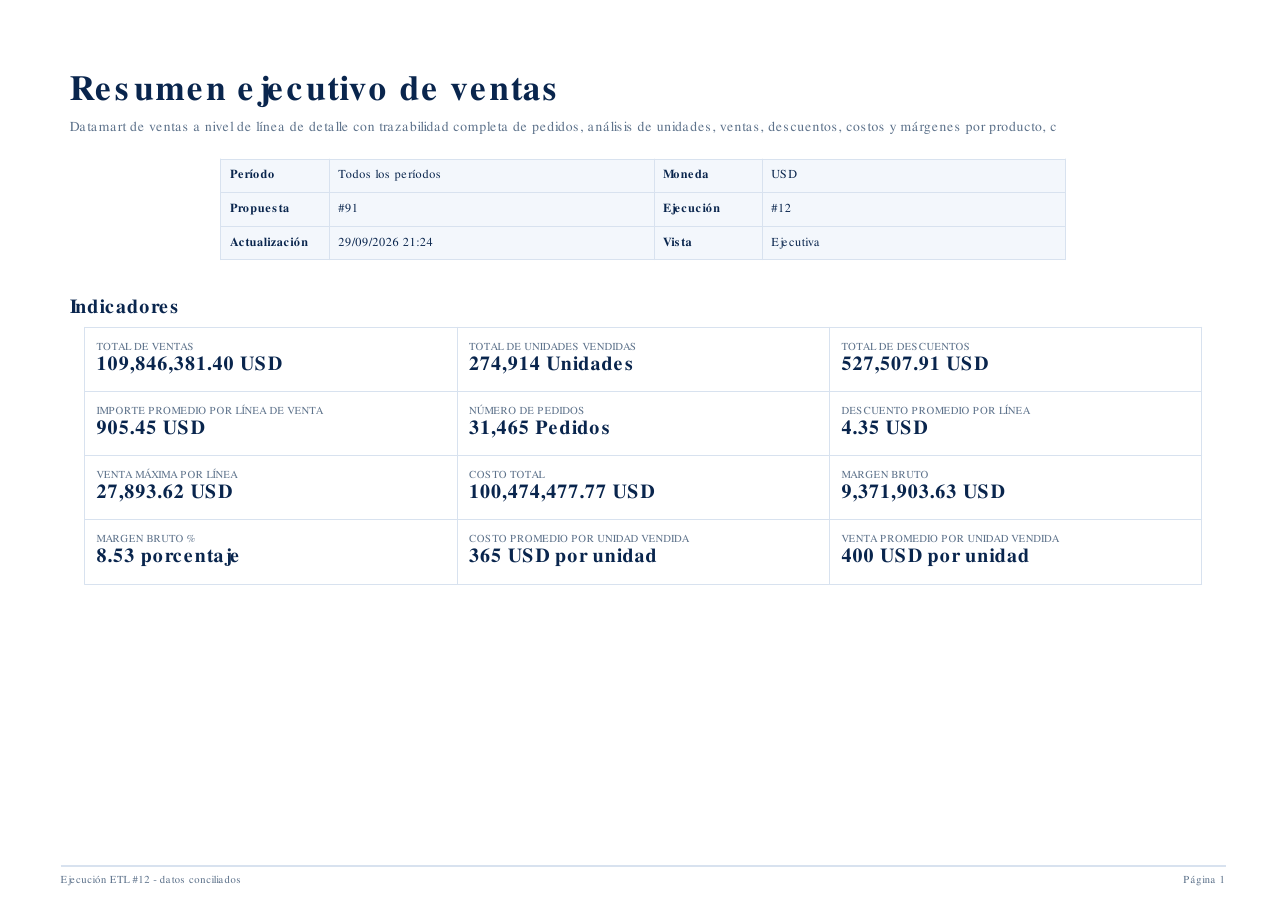
\includegraphics[width=0.92\textwidth]{evidencias/reporte-aw-portada.png}
\caption{Portada PDF post-corrección de AdventureWorks, ejecución 12.}
\end{figure}

\begin{figure}[H]
\centering
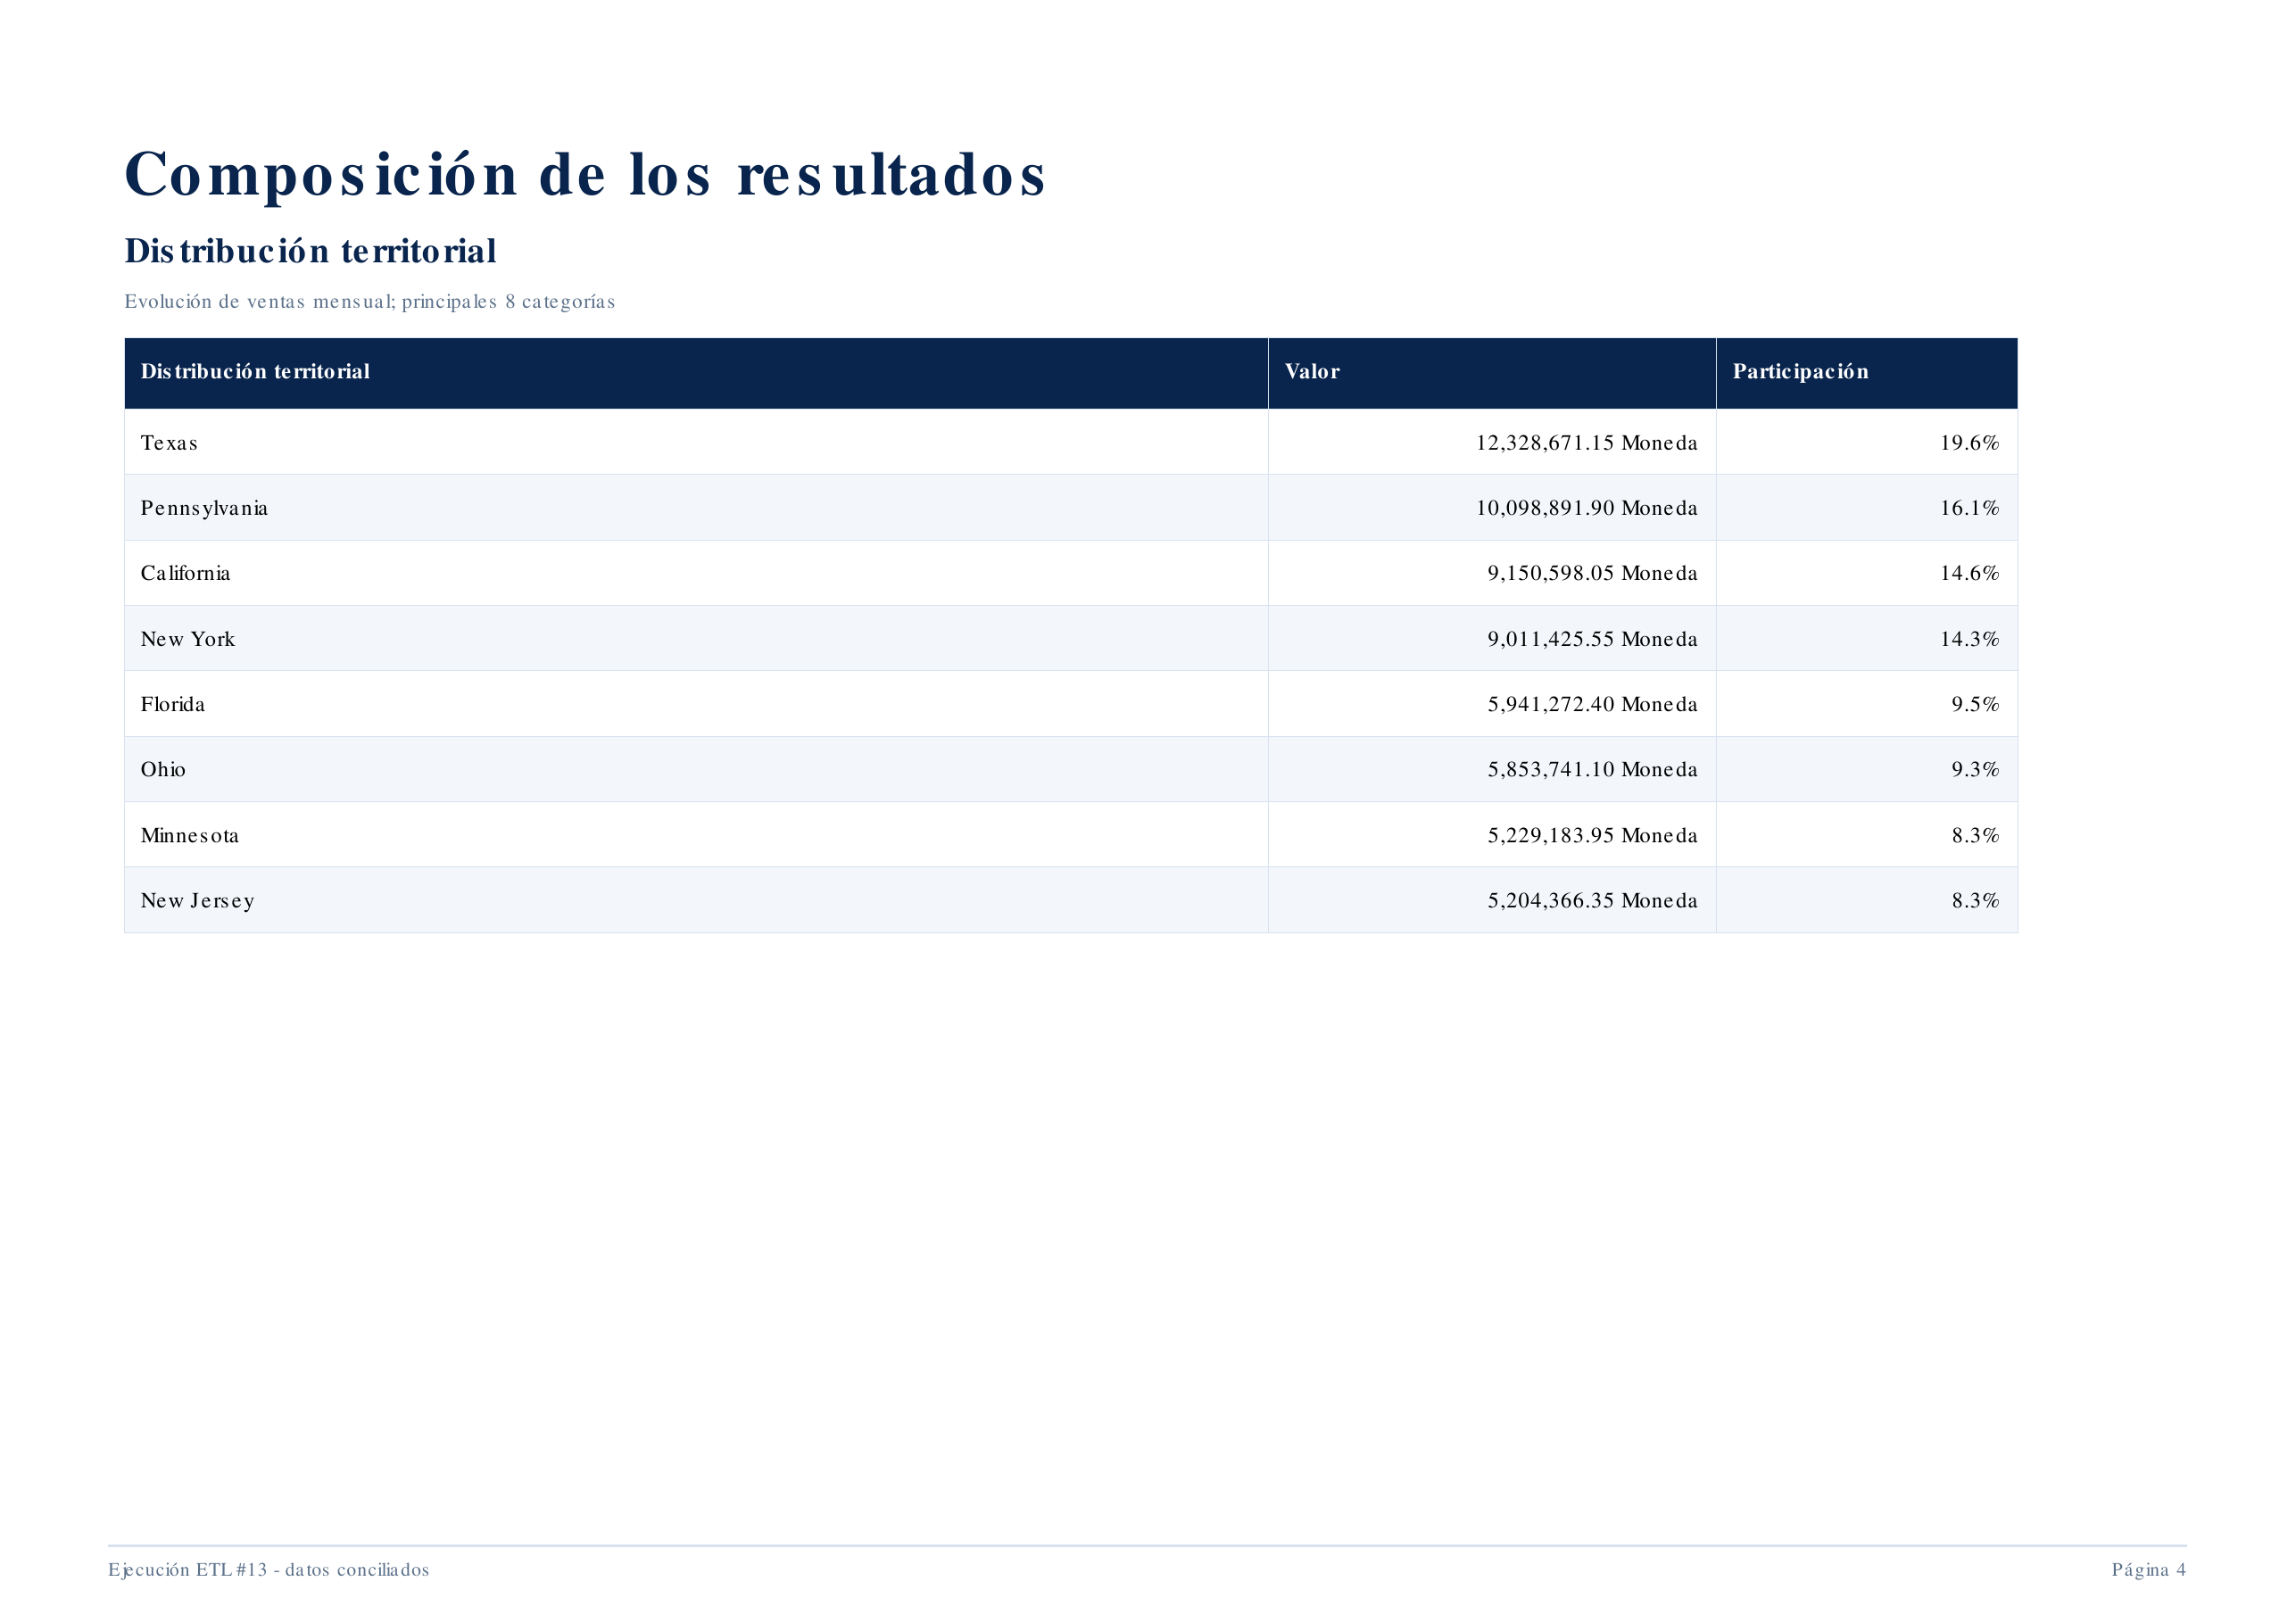
\includegraphics[width=0.92\textwidth]{evidencias/reporte-wwi-territorios.png}
\caption{Tabla territorial PDF post-corrección de WideWorldImporters, ejecución 13.}
\end{figure}

Los Excel se inspeccionaron sin modificarlos. Ambos contienen cuatro hojas: Resumen,
Evolución en el tiempo, Productos líderes y Distribución territorial. Los valores, títulos
y participaciones corresponden a sus respectivas ejecuciones y el área impresa conserva
orientación horizontal.

\begin{figure}[H]
\centering
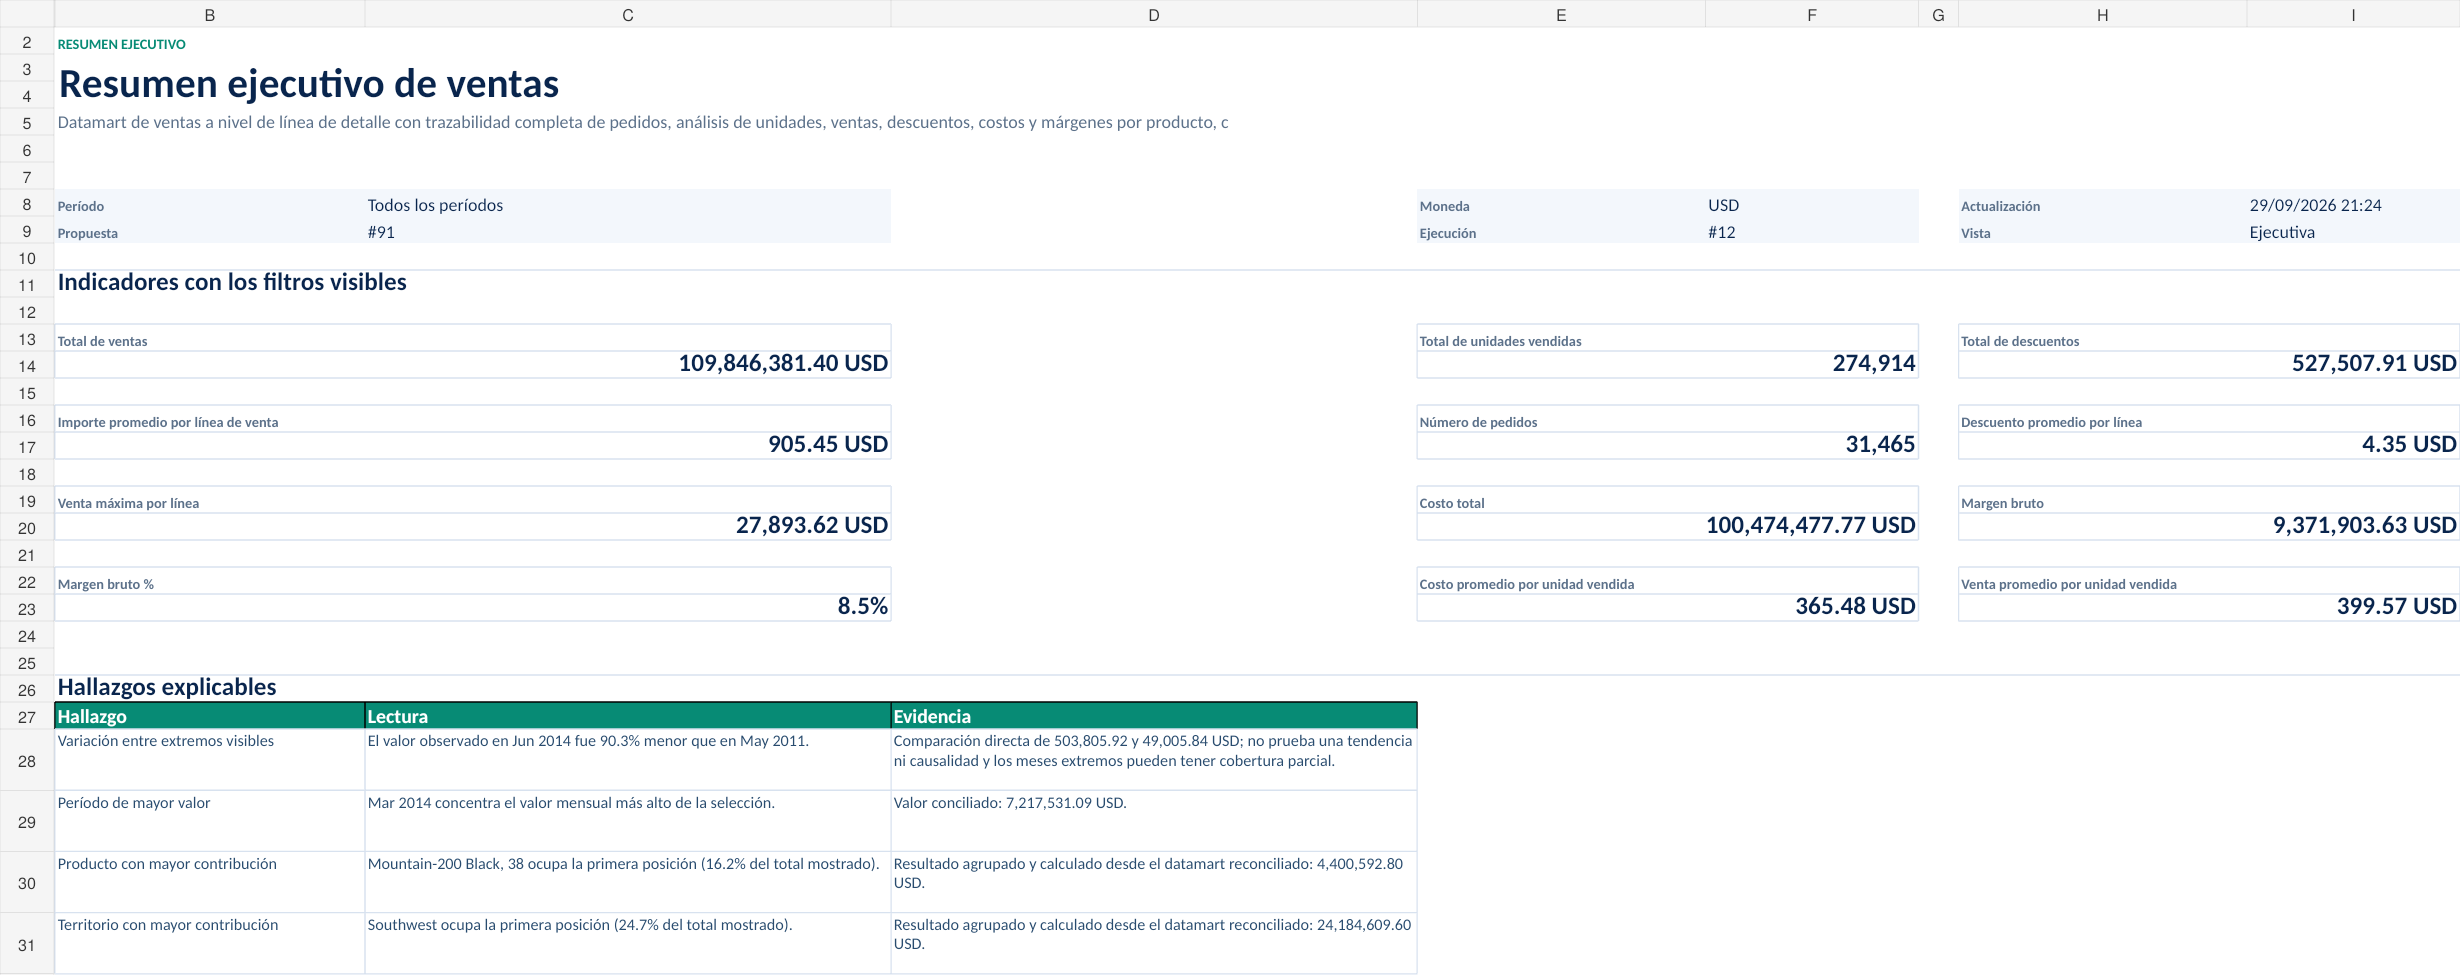
\includegraphics[width=0.98\textwidth]{evidencias/excel-aw-resumen.png}
\caption{Resumen Excel de AdventureWorks inspeccionado visualmente.}
\end{figure}

\begin{figure}[H]
\centering
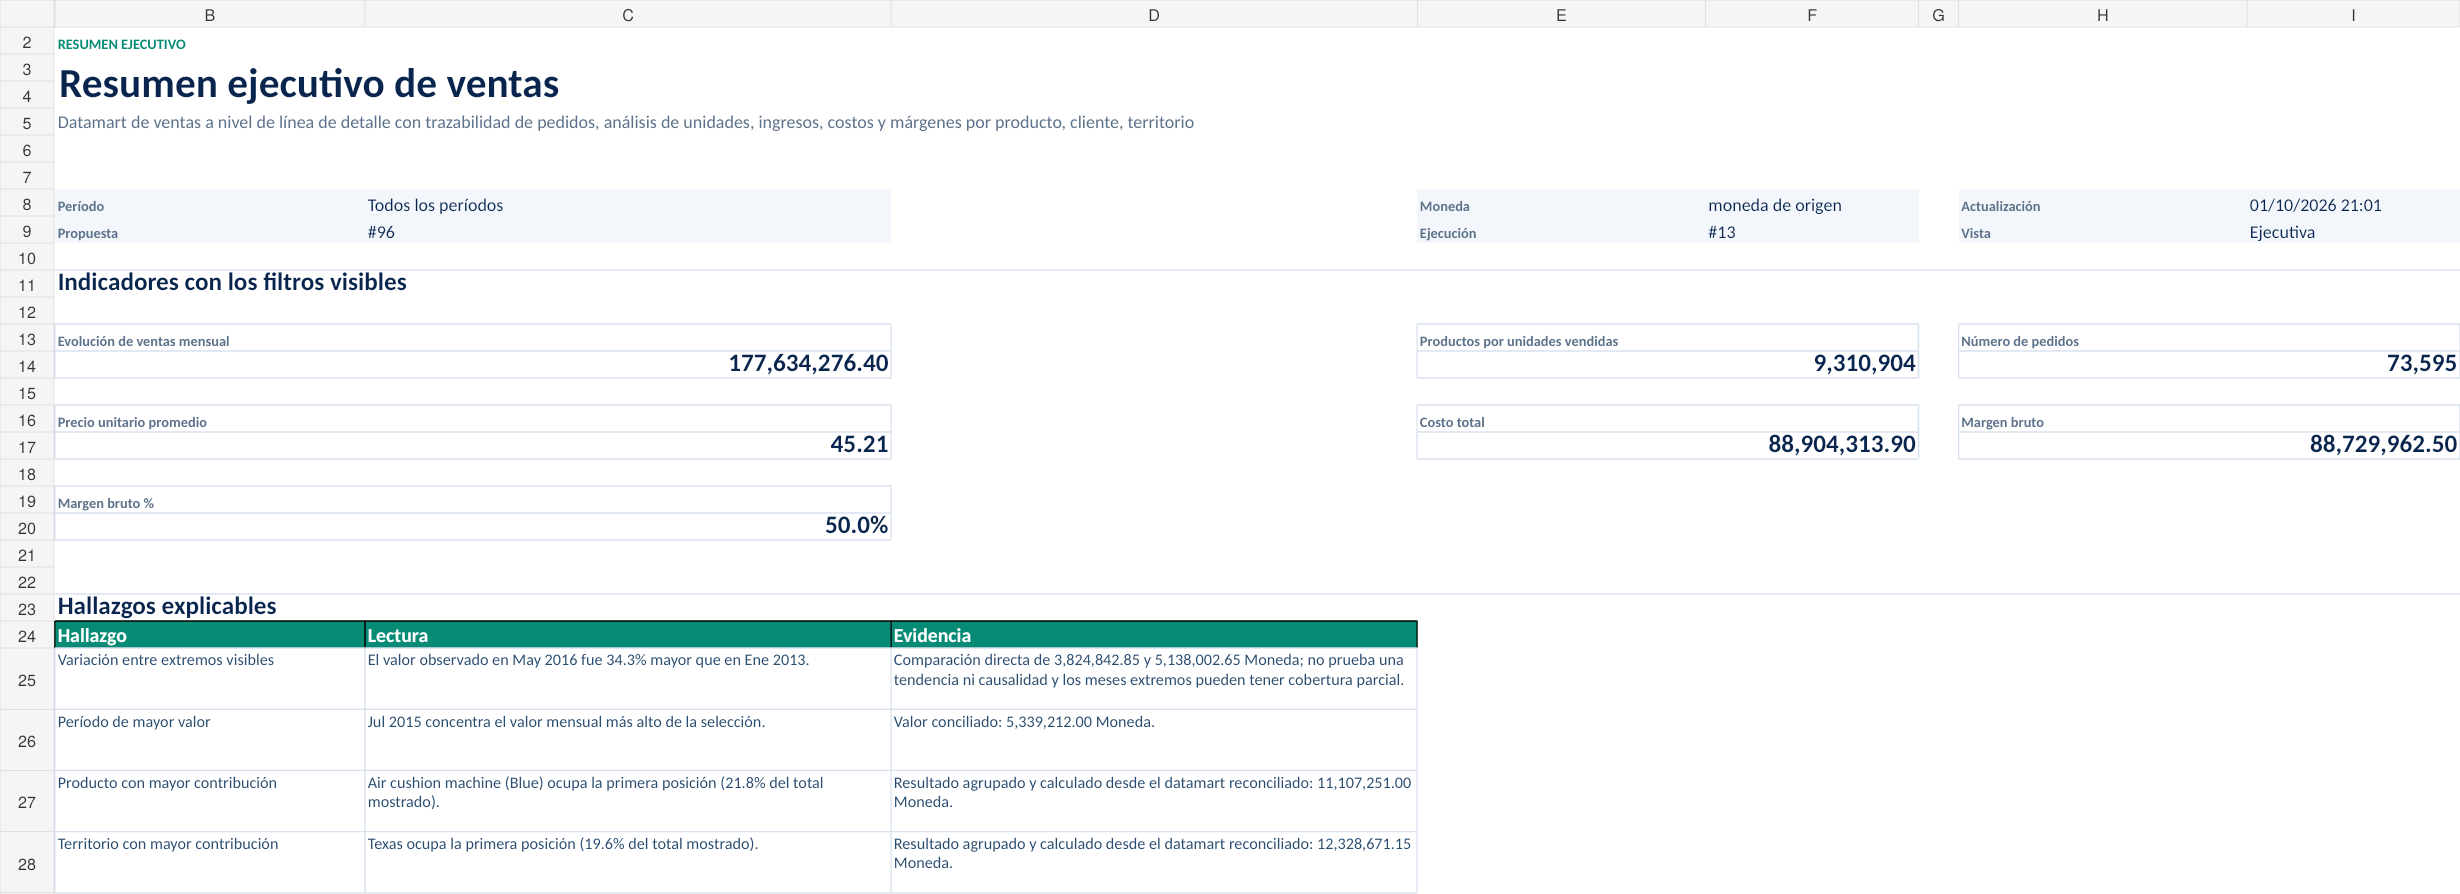
\includegraphics[width=0.98\textwidth]{evidencias/excel-wwi-resumen.png}
\caption{Resumen Excel de WideWorldImporters inspeccionado visualmente.}
\end{figure}

\section{Incidencias encontradas y tratamiento}

\begin{longtable}{@{}p{0.17\textwidth}p{0.24\textwidth}p{0.33\textwidth}p{0.12\textwidth}@{}}
\caption{Defectos encontrados durante la ejecución}\label{tab:defectos}\\
\toprule
Incidencia & Causa & Tratamiento común & Estado \\
\midrule
\endfirsthead
\toprule
Incidencia & Causa & Tratamiento común & Estado \\
\midrule
\endhead
Inicio mostraba AdventureWorks después del cambio & La preparación se consultaba sin conexión explícita. & Se propaga \file{connection\_id} y se reinicia el estado previo. & \fixed \\
Detalle obsoleto al alternar el Explorador & Una respuesta asíncrona anterior podía llegar tarde. & Guardia de petición vigente y remontaje por fuente. & \fixed \\
Preguntas agregadas desaparecieron & El catálogo histórico no se había migrado al nuevo ámbito por fuente. & Migración idempotente al catálogo de la conexión original. & \fixed \\
``Territorio líder'' sin filtro real & Ambigüedad del objeto interpretado por el LLM. & Resolución determinística desde el ranking vigente antes de agregar. & \fixed \\
Valor largo en PDF territorial & La celda numérica usaba texto simple. & Párrafo con alineación y ajuste dentro de la columna. & \fixed \\
\bottomrule
\end{longtable}

\section{Resultados automatizados}

\begin{table}[H]
\centering
\caption{Puerta de calidad repetida después de las correcciones}
\begin{tabularx}{\textwidth}{@{}p{0.34\textwidth}X@{}}
\toprule
Comprobación & Resultado \\
\midrule
Ruff formato & 86 archivos conformes \\
Ruff análisis estático & Sin observaciones \\
Mypy & 56 archivos, sin errores \\
Pytest & 157 pruebas aprobadas; una advertencia de deprecación externa \\
Vitest & 24 pruebas aprobadas en 3 archivos \\
ESLint & Sin advertencias \\
TypeScript y Vite & Compilación de producción aprobada \\
Migraciones & \file{20261001\_17} aplicada como cabeza \\
\bottomrule
\end{tabularx}
\end{table}

\section{Validez, limitaciones y riesgos residuales}

\begin{itemize}
  \item Dos fuentes heterogéneas aumentan la validez del caso respecto de una única base,
  pero no sustituyen pruebas con esquemas empresariales reales adicionales.
  \item La neutralidad se sustenta en contratos y validadores comunes; la calidad del
  borrador del LLM seguirá variando entre proveedores y modelos.
  \item WideWorldImporters no demuestra una divisa única; la etiqueta ``moneda de origen''
  es una limitación explícita y segura.
  \item Las pruebas cubren carga inicial conciliada. Actualización incremental, cambios de
  esquema y concurrencia masiva requieren un incremento posterior.
  \item La advertencia de Starlette no afecta el resultado actual, pero debe atenderse al
  actualizar dependencias.
\end{itemize}

\section{Conclusión para la tesis}

La evidencia respalda que el prototipo implementa un asistente BI multifuente supervisado
para SQL Server. Una misma interfaz trabaja con dos esquemas operacionales distintos, sus
artefactos quedan vinculados a la fuente de origen y las ejecuciones conciliadas producen
tableros, consultas contextuales y reportes independientes.

El principal aporte no es que la IA genere automáticamente cualquier datamart, sino la
combinación de interpretación probabilística con controles determinísticos: metadatos
inmutables, relaciones verificadas, fórmulas permitidas, intervención humana,
materialización versionada y conciliación. Las incidencias detectadas demuestran por qué
esa separación es necesaria: cuando el LLM fue ambiguo o la interfaz conservó estado, el
sistema pudo corregirse en una capa común sin crear una regla específica para una base o
proveedor.

Por tanto, el resultado puede incorporarse como evidencia de verificación del Capítulo III
y como anexo metodológico. La afirmación académicamente defendible es: \emph{el prototipo
mostró portabilidad funcional y aislamiento entre dos fuentes SQL Server del dominio
ventas, bajo un proceso supervisado y reproducible}. No corresponde afirmar todavía
universalidad para cualquier motor o dominio sin pruebas adicionales.

\appendix
\section{Trazabilidad documental}

\begin{tabularx}{\textwidth}{@{}p{0.40\textwidth}X@{}}
\toprule
Documento & Relación con este informe \\
\midrule
Especificación SPR-06-01 & Requisitos y escenarios MS-E2E. \\
Informe del Sprint 6 & Incremento, arquitectura y cierre del Sprint 6. \\
\file{manual-tecnico.pdf} & Operación, verificación y recuperación técnica. \\
Capítulo III de la tesis & Síntesis académica de la propuesta y resultados. \\
\file{bitacora.pdf} & Cronología de decisiones, incidentes y verificaciones. \\
\bottomrule
\end{tabularx}

\end{document}
